
\section{The Interference of Light}

Name \rule{2.0in}{0.1pt}\hfill{}Section \rule{1.0in}{0.1pt}\hfill{}Date
\rule{1.0in}{0.1pt}

\textbf{Objective}

\begin{itemize}
\item To investigate the interference of light waves as they pass through
a set of slits. 
\end{itemize}
\textbf{Apparatus}

\begin{itemize}
\item Laser.
\item Phototransistor for measuring light intensity.
\item Set of narrow slits.
\item {\it DataStudio} 750 Interface.
\item Plumb line.
\end{itemize}
\textbf{Introduction}

In this laboratory you will investigate the interference of light
produced by a laser beam passing through a set of narrow, adjacent
slits. When light passes the slits each opening acts as an independent
source of waves that can overlap one another to produce a distinctive
pattern of bright and dark spots on a screen. The position of the
bright spots depends on the separation of the adjacent slits and the
wavelength of the incident light. 

You can measure this interference pattern with the setup shown below.
A phototransistor is seated behind the narrow opening on top of the large,
metal mount sitting on a rail. The phototransistor can translate the intensity of the
light falling on it into a voltage signal that can be read by the
computer. In addition, the phototransistor can be moved back and
forth on a rotary motion sensor that measures the position of the 
mount.
These two signals can be combined to
make a graph of the intensity as a function of position.

\vspace{0.3cm}
%{\centering \resizebox*{0.75\textwidth}{!}{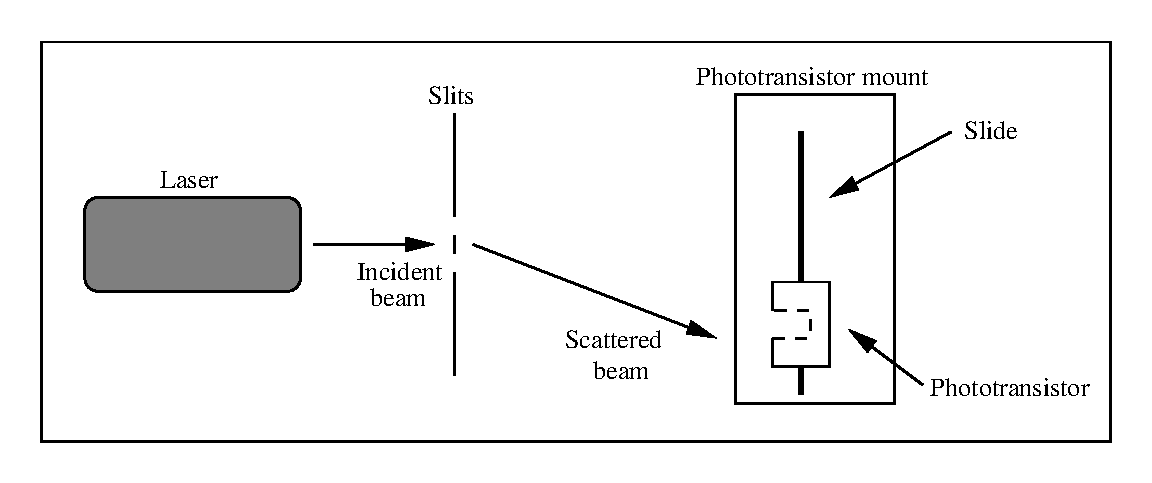
\includegraphics{interference_of_light_fig_1.eps}} \par}
{\centering \resizebox*{0.75\textwidth}{!}{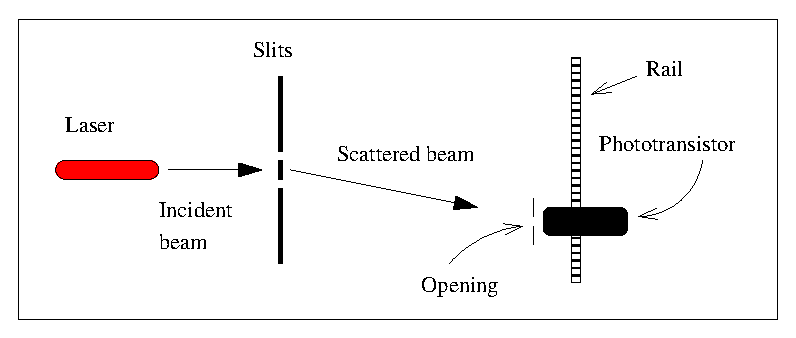
\includegraphics{interference_of_light_fig1b.eps}} \par}
\vspace{0.3cm}

In this unit you will pass light from the laser through slits of known
separation and use the interference pattern to determine the wavelength
of the light.

\textbf{Activity 1: An Alternative View}

Isaac Newton believed that light was made up of small, unseen particles
that obeyed (surprisingly enough!) Newton s Laws. This view is known
as the corpuscular theory. We want to consider how this model of light
predicts different behavior from the wave theory.

\vspace{35mm}
(a) Consider a laser beam shining on a circular hole. If a beam of
light consisted of small, unseen particles that behaved as tiny billiard
balls what would see on a screen that is downstream from the circular
hole? A sketch might be useful here.
\vspace{1.5in}

(b) Now consider the same laser beam shining on a pair of narrow slits.
What would you see on a screen downstream from the slits if light
wire made of corpuscles?
\vspace{30mm}

For the questions above you should have predicted that the laser would
form a single bright spot (for part a) or a double spot (for part
b). The experiment you are about to perform provided compelling evidence
that Newton s corpuscular theory was wrong. 

\textbf{Activity 2: The Interference of Light }

(a) You are now ready to turn on the laser. DO NOT LOOK DIRECTLY INTO
THE BEAM OR POINT THE LASER CARELESSLY ABOUT THE ROOM. Turn on the
laser and you should see the bright red spot of the beam striking
the wall. You should have a glass plate with a green border and several
different slit arrangements on it. Place the opening in the center
of the plate in the path of the laser beam. The adjacent slits in
the center hole are 0.03295 mm apart. What do you see? 
\vspace{15mm}

(b) Position the glass plate about 30-40 cm from the phototransistor
mount with the central maximum (the brightest spot) 
striking the center hole. Measure and record this
distance. You may find it useful to use the plumb line to measure
this distance.
The phototransistor sits about 25.4 mm behind the opening.
\vspace{15mm}

(c) Position the phototransistor mount so the interference pattern
is at the same height as the opening in the center of the
phototransistor mount. The phototransistor is mounted behind this hole.
To make accurate measurements it is important
to carefully determine the geometry of your setup. Check to see if
the slits and the phototransistor mount are perpendicular to the incident
laser beam. 
You want to make sure the phototransistor can {}``see'' as many
bright spots as possible. Carefully slide the phototransistor mount back and forth to
make sure the it stays centered on the interference pattern.
Start the ``Interference'' activity in the {\bf 132 Workshop} folder. 
When you are ready, click {\bf Start}
and slowly push the phototransistor from one side of the slide to
the other. Move carefully and take about 4-5 seconds to complete the
motion. Click {\bf Stop}.
When data acquisition is complete you will see a graph representing
the intensity reading versus the position reading. You should see
several distinct peaks. This graph is the interference pattern. If
you do not see this pattern consult your instructor. Make a hardcopy
of this graph and attach it to the unit.

(d) Is the spacing between the intensity peaks constant? Is the intensity
of each peak the same? Does it appear that any peaks are missing?
The more peaks you see the more (and hopefully better) data you can collect.
There is a button on top of the phototransistor labeled ``Gain'' which changes
the size of the intensity signal.
Trying changing this setting to see if you can get more peaks in your spectrum.
\vspace{15mm}

(e) When you are satisfied with the quality of your spectrum record the position of 
each peak in the table below.
Use the
{\bf Smart Tool} to accurately read off the peak positions by clicking on the
appropriate button along the top of the graph. A set of cross-hairs will appear on the
plot. Grab the cross-hairs by clicking on them and dragging them to the point you want
to measure.
The coordinates will be printed by the cross-hairs.
Turn off the laser when you are finished.

\vspace{0.3cm}
{\centering \begin{tabular}{|c|c|}
\hline 
Position Reading (m)&
Change in Reading (m)\\
\hline
\hline 
&
\\
\hline 
&
\\
\hline 
&
\\
\hline 
&
\\
\hline 
&
\\
\hline 
&
\\
\hline 
&
\\
\hline
\end{tabular}\par}
\vspace{0.3cm}

\textbf{Activity 3: Determining the Wavelength of the Laser }

(a) For the data you recorded in the previous activity calculate the
difference between each pair of adjacent readings and record
it in your data table.

(b) Calculate the average and standard deviation of the separation between 
adjacent peaks.
\vspace{15mm}

(c) The position of the interference maxima can be described by

\[
y_{m}=\frac{\lambda D}{d}m\]


where y\( _{m} \) is the distance of a bright spot from the central
maximum (the distance along the slide in this experiment) and D is
the distance from the slits to the phototransistor. The quantity d
is the slit separation, \( \lambda  \) is the wavelength of the light,
and m is the order of the bright spot. Generate an expression for
the distance between adjacent bright spots.
\vspace{15mm}

(d) Use the expression you calculated above and the average separation
between bright spots to calculate the wavelength of the laser light.
Compare your result with the expected value of 6328 angstroms. Are
the peaks of the interference pattern the same intensity? Describe
the pattern you observe.
\vspace{30mm}

\newpage

(e) Collect the results for the wavelength from the other teams in class
and calculate the average and standard deviation. Record the result here.
Are you results consistent with the class results? Why or why not?
\vspace{30mm}

(f) Recall the earlier discussion of Newton's corpuscular theory of
light. Does your data support Newton's theory or the wave theory?
Why?\vspace{15mm}

